\begin{figure}[h]
    \centering
    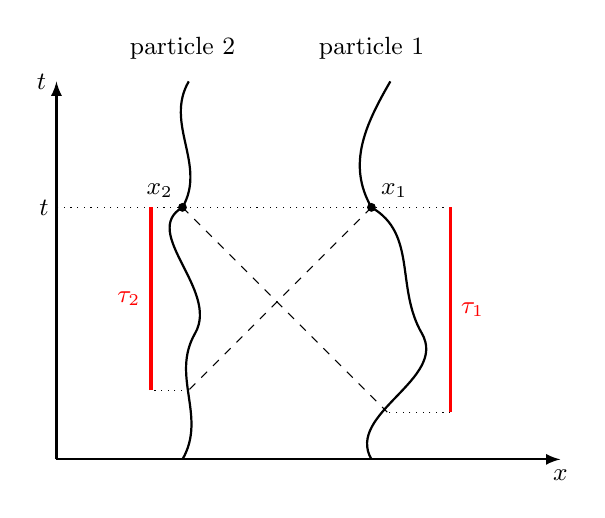
\begin{tikzpicture}[>=latex, every node/.style={font=\small}, scale=0.8]
  % Axes
  \draw[thick, ->](0,0) -- (0,6) node[left] {$t$};
  \draw[thick, ->] (0,0) -- (8,0) node[below] {$x$};

  % Particle 2 worldline (left)
  \coordinate (P2start) at (2,0);
  \coordinate (P2mid)   at (2.2,2);
  \coordinate (P2evt)   at (2,4);
  \coordinate (P2top)   at (2.1,6);
  \draw[thick] (P2start) to[out=60,in=240] (P2mid) 
                to[out=60,in=210] (P2evt) 
                to[out=60,in=240] (P2top);

  % Particle 1 worldline (right)
  \coordinate (P1start) at (5,0);
  \coordinate (P1mid)   at (5.8,2);
  \coordinate (P1evt)   at (5,4);
  \coordinate (P1top)   at (5.3,6);
  \draw[thick] (P1start) to[out=120,in=-60] (P1mid) 
                to[out=120,in=-30] (P1evt) 
                to[out=120,in=-120] (P1top);

  % Events x1 and x2
  \fill (P1evt) circle (2pt) node[above right] {$x_1$};
  \fill (P2evt) circle (2pt) node[above left]  {$x_2$};

  % Dotted equal-time slice
  \draw[dotted] (6.25, 4) -- (0,4);
  \node at (-0.2, 4) {\(t\)};

  \draw[dotted] (6.25, 0.75) -- (5.25,0.75);
  \draw[dotted] (2.1, 1.1) -- (1.5, 1.1);
  

  % Spacelike dashed path
  \draw[dashed] (P1evt) -- (2.1,1.1);
  \draw[dashed] (P2evt) -- (5.25,0.75);


  % Constant-time slices (red)
  \draw[red,very thick] (1.5,1.1) -- (1.5,4)
    node[left,midway] {$\tau_2$};
  \draw[red,very thick] (6.25, 0.75) -- (6.25, 4)
    node[right,midway] {$\tau_1$};

  % Labels for worldlines
  \node at (2,6.2) [above] {particle 2};
  \node at (5,6.2) [above] {particle 1};
\end{tikzpicture}
\end{figure}